\section{System Engineering and Verification Architecture}
\label{sec:arch}

Protocol CRS, tool requirements and experiment requirements stay in separate
layers. Row count does not prove a method. A concrete owned trace is source
unit \texttt{SU-ARINC-615A-3-SECTION-6-3-2-}\allowbreak
\texttt{SEQUENCE-CHART-A-E007-7726A816FFE7}
\(\to\) CRS-M1-00365/00366/00367 \(\to\) LUR write-order constraint \(\to\)
planned Test/Analysis verification case \(\to\) later tool module. The IDs are
real bound-M1 identifiers. \texttt{satisfy}/\texttt{verify} in the SysML view
are model relations, not executed verification. No standard figure is reprinted.

Two machines must not be merged. \(M_{\mathrm{sess}}\) selects from
\(S\subseteq A(q)\), charges once, updates \(H\) and returns a named stop.
\(M_{\mathrm{prot}}\) is the UPLOAD/INFORMATION black box. Execute issues a
stimulus and obtains a raw execution record. Interpretation, not the network
port, produces the compatible class \(I_z\) and hypothesis survivors.

\begin{figure}[!ht]
\centering
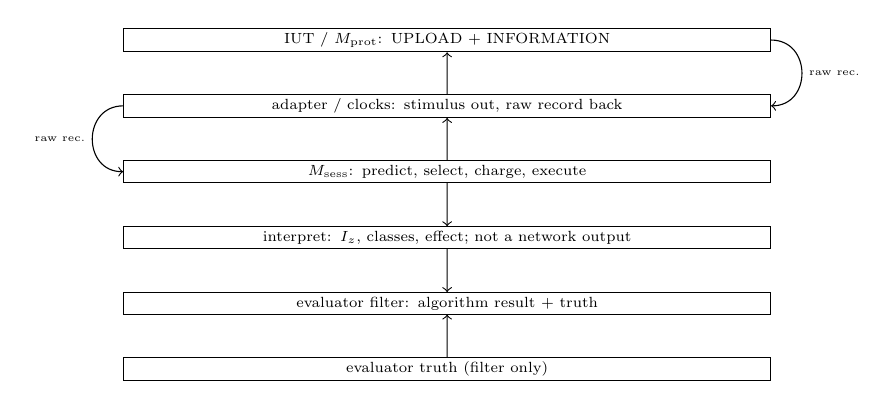
\begin{tikzpicture}[scale=0.76,transform shape,font=\scriptsize,box/.style={draw,align=center,inner sep=2pt,text width=0.88\columnwidth}]
\node[box] (iut) at (0,4.4) {IUT / \(M_{\mathrm{prot}}\): UPLOAD + INFORMATION};
\node[box] (adp) at (0,3.3) {adapter / clocks: stimulus out, raw record back};
\node[box] (sess) at (0,2.2) {\(M_{\mathrm{sess}}\): predict, select, charge, execute};
\node[box] (interp) at (0,1.1) {interpret: \(I_z\), classes, effect; not a network output};
\node[box] (filt) at (0,0.0) {evaluator filter: algorithm result + truth};
\node[box] (truth) at (0,-1.1) {evaluator truth (filter only)};
\draw[->] (sess) -- (adp);
\draw[->] (adp) -- (iut);
\draw[->] (iut.east) to[out=0,in=0,looseness=1.6] node[right,font=\tiny] {raw rec.} (adp.east);
\draw[->] (adp.west) to[out=180,in=180,looseness=1.6] node[left,font=\tiny] {raw rec.} (sess.west);
\draw[->] (sess) -- (interp);
\draw[->] (interp) -- (filt);
\draw[->] (truth) -- (filt);
\end{tikzpicture}
\caption{Context derived from FIG-CL-TAV-01/07. Stimulus and raw records share
ports. Truth enters only the evaluator filter, never select, predict, history
or execute.}
\label{fig:arch}
\end{figure}

Expanded CRS leaves do not add FIND or DOWNLOAD transitions to
\(M_{\mathrm{prot}}\).
\phbox{PH-IMPL-KERNEL}{IMPLEMENTATION-DETAIL}{Core estimators, pairing solvers
and the history representation remain interface contracts and are not deployed.}
